
%% bare_conf.tex
%% V1.3
%% 2007/01/11
%% by Michael Shell
%% See:
%% http://www.michaelshell.org/
%% for current contact information.
%%
%% This is a skeleton file demonstrating the use of IEEEtran.cls
%% (requires IEEEtran.cls version 1.7 or later) with an IEEE conference paper.
%%
%% Support sites:
%% http://www.michaelshell.org/tex/ieeetran/
%% http://www.ctan.org/tex-archive/macros/latex/contrib/IEEEtran/
%% and
%% http://www.ieee.org/

%%*************************************************************************
%% Legal Notice:
%% This code is offered as-is without any warranty either expressed or
%% implied; without even the implied warranty of MERCHANTABILITY or
%% FITNESS FOR A PARTICULAR PURPOSE! 
%% User assumes all risk.
%% In no event shall IEEE or any contributor to this code be liable for
%% any damages or losses, including, but not limited to, incidental,
%% consequential, or any other damages, resulting from the use or misuse
%% of any information contained here.
%%
%% All comments are the opinions of their respective authors and are not
%% necessarily endorsed by the IEEE.
%%
%% This work is distributed under the LaTeX Project Public License (LPPL)
%% ( http://www.latex-project.org/ ) version 1.3, and may be freely used,
%% distributed and modified. A copy of the LPPL, version 1.3, is included
%% in the base LaTeX documentation of all distributions of LaTeX released
%% 2003/12/01 or later.
%% Retain all contribution notices and credits.
%% ** Modified files should be clearly indicated as such, including  **
%% ** renaming them and changing author support contact information. **
%%
%% File list of work: IEEEtran.cls, IEEEtran_HOWTO.pdf, bare_adv.tex,
%%                    bare_conf.tex, bare_jrnl.tex, bare_jrnl_compsoc.tex
%%*************************************************************************

% *** Authors should verify (and, if needed, correct) their LaTeX system  ***
% *** with the testflow diagnostic prior to trusting their LaTeX platform ***
% *** with production work. IEEE's font choices can trigger bugs that do  ***
% *** not appear when using other class files.                            ***
% The testflow support page is at:
% http://www.michaelshell.org/tex/testflow/



% Note that the a4paper option is mainly intended so that authors in
% countries using A4 can easily print to A4 and see how their papers will
% look in print - the typesetting of the document will not typically be
% affected with changes in paper size (but the bottom and side margins will).
% Use the testflow package mentioned above to verify correct handling of
% both paper sizes by the user's LaTeX system.
%
% Also note that the "draftcls" or "draftclsnofoot", not "draft", option
% should be used if it is desired that the figures are to be displayed in
% draft mode.
%
\documentclass[conference]{IEEEtran}
% Add the compsoc option for Computer Society conferences.
%
% If IEEEtran.cls has not been installed into the LaTeX system files,
% manually specify the path to it like:
% \documentclass[conference]{../sty/IEEEtran}





% Some very useful LaTeX packages include:
% (uncomment the ones you want to load)


% *** MISC UTILITY PACKAGES ***
%
%\usepackage{ifpdf}
% Heiko Oberdiek's ifpdf.sty is very useful if you need conditional
% compilation based on whether the output is pdf or dvi.
% usage:
% \ifpdf
%   % pdf code
% \else
%   % dvi code
% \fi
% The latest version of ifpdf.sty can be obtained from:
% http://www.ctan.org/tex-archive/macros/latex/contrib/oberdiek/
% Also, note that IEEEtran.cls V1.7 and later provides a builtin
% \ifCLASSINFOpdf conditional that works the same way.
% When switching from latex to pdflatex and vice-versa, the compiler may
% have to be run twice to clear warning/error messages.






% *** CITATION PACKAGES ***
%
\usepackage{cite}
% cite.sty was written by Donald Arseneau
% V1.6 and later of IEEEtran pre-defines the format of the cite.sty package
% \cite{} output to follow that of IEEE. Loading the cite package will
% result in citation numbers being automatically sorted and properly
% "compressed/ranged". e.g., [1], [9], [2], [7], [5], [6] without using
% cite.sty will become [1], [2], [5]--[7], [9] using cite.sty. cite.sty's
% \cite will automatically add leading space, if needed. Use cite.sty's
% noadjust option (cite.sty V3.8 and later) if you want to turn this off.
% cite.sty is already installed on most LaTeX systems. Be sure and use
% version 4.0 (2003-05-27) and later if using hyperref.sty. cite.sty does
% not currently provide for hyperlinked citations.
% The latest version can be obtained at:
% http://www.ctan.org/tex-archive/macros/latex/contrib/cite/
% The documentation is contained in the cite.sty file itself.






% *** GRAPHICS RELATED PACKAGES ***
%
\ifCLASSINFOpdf
  % \usepackage[pdftex]{graphicx}
  % declare the path(s) where your graphic files are
  % \graphicspath{{../pdf/}{../jpeg/}}
  % and their extensions so you won't have to specify these with
  % every instance of \includegraphics
  % \DeclareGraphicsExtensions{.pdf,.jpeg,.png}
\else
  % or other class option (dvipsone, dvipdf, if not using dvips). graphicx
  % will default to the driver specified in the system graphics.cfg if no
  % driver is specified.
  % \usepackage[dvips]{graphicx}
  % declare the path(s) where your graphic files are
  % \graphicspath{{../eps/}}
  % and their extensions so you won't have to specify these with
  % every instance of \includegraphics
  % \DeclareGraphicsExtensions{.eps}
\fi
% graphicx was written by David Carlisle and Sebastian Rahtz. It is
% required if you want graphics, photos, etc. graphicx.sty is already
% installed on most LaTeX systems. The latest version and documentation can
% be obtained at: 
% http://www.ctan.org/tex-archive/macros/latex/required/graphics/
% Another good source of documentation is "Using Imported Graphics in
% LaTeX2e" by Keith Reckdahl which can be found as epslatex.ps or
% epslatex.pdf at: http://www.ctan.org/tex-archive/info/
%
% latex, and pdflatex in dvi mode, support graphics in encapsulated
% postscript (.eps) format. pdflatex in pdf mode supports graphics
% in .pdf, .jpeg, .png and .mps (metapost) formats. Users should ensure
% that all non-photo figures use a vector format (.eps, .pdf, .mps) and
% not a bitmapped formats (.jpeg, .png). IEEE frowns on bitmapped formats
% which can result in "jaggedy"/blurry rendering of lines and letters as
% well as large increases in file sizes.
%
% You can find documentation about the pdfTeX application at:
% http://www.tug.org/applications/pdftex





% *** MATH PACKAGES ***
%
%\usepackage[cmex10]{amsmath}
% A popular package from the American Mathematical Society that provides
% many useful and powerful commands for dealing with mathematics. If using
% it, be sure to load this package with the cmex10 option to ensure that
% only type 1 fonts will utilized at all point sizes. Without this option,
% it is possible that some math symbols, particularly those within
% footnotes, will be rendered in bitmap form which will result in a
% document that can not be IEEE Xplore compliant!
%
% Also, note that the amsmath package sets \interdisplaylinepenalty to 10000
% thus preventing page breaks from occurring within multiline equations. Use:
%\interdisplaylinepenalty=2500
% after loading amsmath to restore such page breaks as IEEEtran.cls normally
% does. amsmath.sty is already installed on most LaTeX systems. The latest
% version and documentation can be obtained at:
% http://www.ctan.org/tex-archive/macros/latex/required/amslatex/math/





% *** SPECIALIZED LIST PACKAGES ***
%
%\usepackage{algorithmic}
% algorithmic.sty was written by Peter Williams and Rogerio Brito.
% This package provides an algorithmic environment fo describing algorithms.
% You can use the algorithmic environment in-text or within a figure
% environment to provide for a floating algorithm. Do NOT use the algorithm
% floating environment provided by algorithm.sty (by the same authors) or
% algorithm2e.sty (by Christophe Fiorio) as IEEE does not use dedicated
% algorithm float types and packages that provide these will not provide
% correct IEEE style captions. The latest version and documentation of
% algorithmic.sty can be obtained at:
% http://www.ctan.org/tex-archive/macros/latex/contrib/algorithms/
% There is also a support site at:
% http://algorithms.berlios.de/index.html
% Also of interest may be the (relatively newer and more customizable)
% algorithmicx.sty package by Szasz Janos:
% http://www.ctan.org/tex-archive/macros/latex/contrib/algorithmicx/




% *** ALIGNMENT PACKAGES ***
%
%\usepackage{array}
% Frank Mittelbach's and David Carlisle's array.sty patches and improves
% the standard LaTeX2e array and tabular environments to provide better
% appearance and additional user controls. As the default LaTeX2e table
% generation code is lacking to the point of almost being broken with
% respect to the quality of the end results, all users are strongly
% advised to use an enhanced (at the very least that provided by array.sty)
% set of table tools. array.sty is already installed on most systems. The
% latest version and documentation can be obtained at:
% http://www.ctan.org/tex-archive/macros/latex/required/tools/


%\usepackage{mdwmath}
%\usepackage{mdwtab}
% Also highly recommended is Mark Wooding's extremely powerful MDW tools,
% especially mdwmath.sty and mdwtab.sty which are used to format equations
% and tables, respectively. The MDWtools set is already installed on most
% LaTeX systems. The lastest version and documentation is available at:
% http://www.ctan.org/tex-archive/macros/latex/contrib/mdwtools/


% IEEEtran contains the IEEEeqnarray family of commands that can be used to
% generate multiline equations as well as matrices, tables, etc., of high
% quality.


%\usepackage{eqparbox}
% Also of notable interest is Scott Pakin's eqparbox package for creating
% (automatically sized) equal width boxes - aka "natural width parboxes".
% Available at:
% http://www.ctan.org/tex-archive/macros/latex/contrib/eqparbox/





% *** SUBFIGURE PACKAGES ***
%\usepackage[tight,footnotesize]{subfigure}
% subfigure.sty was written by Steven Douglas Cochran. This package makes it
% easy to put subfigures in your figures. e.g., "Figure 1a and 1b". For IEEE
% work, it is a good idea to load it with the tight package option to reduce
% the amount of white space around the subfigures. subfigure.sty is already
% installed on most LaTeX systems. The latest version and documentation can
% be obtained at:
% http://www.ctan.org/tex-archive/obsolete/macros/latex/contrib/subfigure/
% subfigure.sty has been superceeded by subfig.sty.



%\usepackage[caption=false]{caption}
%\usepackage[font=footnotesize]{subfig}
% subfig.sty, also written by Steven Douglas Cochran, is the modern
% replacement for subfigure.sty. However, subfig.sty requires and
% automatically loads Axel Sommerfeldt's caption.sty which will override
% IEEEtran.cls handling of captions and this will result in nonIEEE style
% figure/table captions. To prevent this problem, be sure and preload
% caption.sty with its "caption=false" package option. This is will preserve
% IEEEtran.cls handing of captions. Version 1.3 (2005/06/28) and later 
% (recommended due to many improvements over 1.2) of subfig.sty supports
% the caption=false option directly:
%\usepackage[caption=false,font=footnotesize]{subfig}
%
% The latest version and documentation can be obtained at:
% http://www.ctan.org/tex-archive/macros/latex/contrib/subfig/
% The latest version and documentation of caption.sty can be obtained at:
% http://www.ctan.org/tex-archive/macros/latex/contrib/caption/




% *** FLOAT PACKAGES ***
%
%\usepackage{fixltx2e}
% fixltx2e, the successor to the earlier fix2col.sty, was written by
% Frank Mittelbach and David Carlisle. This package corrects a few problems
% in the LaTeX2e kernel, the most notable of which is that in current
% LaTeX2e releases, the ordering of single and double column floats is not
% guaranteed to be preserved. Thus, an unpatched LaTeX2e can allow a
% single column figure to be placed prior to an earlier double column
% figure. The latest version and documentation can be found at:
% http://www.ctan.org/tex-archive/macros/latex/base/



%\usepackage{stfloats}
% stfloats.sty was written by Sigitas Tolusis. This package gives LaTeX2e
% the ability to do double column floats at the bottom of the page as well
% as the top. (e.g., "\begin{figure*}[!b]" is not normally possible in
% LaTeX2e). It also provides a command:
%\fnbelowfloat
% to enable the placement of footnotes below bottom floats (the standard
% LaTeX2e kernel puts them above bottom floats). This is an invasive package
% which rewrites many portions of the LaTeX2e float routines. It may not work
% with other packages that modify the LaTeX2e float routines. The latest
% version and documentation can be obtained at:
% http://www.ctan.org/tex-archive/macros/latex/contrib/sttools/
% Documentation is contained in the stfloats.sty comments as well as in the
% presfull.pdf file. Do not use the stfloats baselinefloat ability as IEEE
% does not allow \baselineskip to stretch. Authors submitting work to the
% IEEE should note that IEEE rarely uses double column equations and
% that authors should try to avoid such use. Do not be tempted to use the
% cuted.sty or midfloat.sty packages (also by Sigitas Tolusis) as IEEE does
% not format its papers in such ways.





% *** PDF, URL AND HYPERLINK PACKAGES ***
%
\usepackage{url}
% url.sty was written by Donald Arseneau. It provides better support for
% handling and breaking URLs. url.sty is already installed on most LaTeX
% systems. The latest version can be obtained at:
% http://www.ctan.org/tex-archive/macros/latex/contrib/misc/
% Read the url.sty source comments for usage information. Basically,
% \url{my_url_here}.





% *** Do not adjust lengths that control margins, column widths, etc. ***
% *** Do not use packages that alter fonts (such as pslatex).         ***
% There should be no need to do such things with IEEEtran.cls V1.6 and later.
% (Unless specifically asked to do so by the journal or conference you plan
% to submit to, of course. )

\usepackage{verbatim}
\usepackage{amsmath}
\usepackage{amssymb}
\usepackage{caption}
\usepackage{subcaption,balance}
%\usepackage[sort,compress,noadjust]{cite}

% self defined
\usepackage{dsfont}
\usepackage{tabularx}
\usepackage{csquotes}
\usepackage{algorithm}
\usepackage{algpseudocode}
\algtext*{EndFunction}% Remove "end function" text

\newtheorem{thm}{Theorem}
\DeclareMathOperator{\height}{height}
\DeclareMathOperator{\amv}{AMV}
\DeclareMathOperator{\mv}{MV}
\DeclareMathOperator{\prio}{priority}
\DeclareMathOperator{\offset}{offset}

\DeclareMathOperator{\drop}{Drop}
\DeclareMathOperator{\forward}{Forward}
\DeclareMathOperator{\true}{true}
\DeclareMathOperator{\false}{false}

\def\TReg{\textsuperscript{\textregistered}}
\def\TCop{\textsuperscript{\textcopyright}}
\def\TTra{\textsuperscript{\texttrademark}}

%\newcommand{\imgscale}{0.545}
\newcommand{\imgscale}{0.5}
\newcommand{\imgwidth}{0.65}
\newcommand{\imgspace}{\vspace*{-0.25cm}}
\newcommand{\actset}{\mathcal{ACT}}
\newcommand{\priotree}{PT}
\ifCLASSINFOpdf
  \usepackage[pdftex]{graphicx}
\else
\fi

% correct bad hyphenation here
\hyphenation{op-tical net-works semi-conduc-tor}

\renewcommand{\algorithmiccomment}[1]{{// #1}}

\begin{document}
%
% paper title
% can use linebreaks \\ within to get better formatting as desired
\title{Measurements and Optimizations with Just-In-Time Code Generation on the OpenFlow Reference Implementation}

%\begin{comment}
%\author{\IEEEauthorblockN{\hspace*{0.0cm}Samuel Brack}
%% \IEEEauthorblockA{Computer Engineering Group\\
%% Humboldt University\\
%% Berlin, Germany}
%\and
%\IEEEauthorblockN{\hspace*{-0.8cm}Sven Hager}
%\IEEEauthorblockA{~\\
%\hspace*{-1.0cm}Computer Engineering Group\\
%\hspace*{-1.0cm}Humboldt University of Berlin, Germany\\
%% Berlin, Germany\\
%\hspace*{-1.0cm}$\text{Email: } \lbrace \text{bracksam, hagersve, scheuermann}\rbrace$@informatik.hu-berlin.de}
%\and
%\IEEEauthorblockN{\hspace*{-1.8cm}Bj{\"o}rn Scheuermann}
%}
%\end{comment}

\author{\IEEEauthorblockN{Samuel Brack}
\IEEEauthorblockA{Computer Engineering Group, Humboldt University of Berlin, Germany\\
samuel.brack@informatik.hu-berlin.de}
}

% author names and affiliations
% use a multiple column layout for up to three different
% affiliations
%%%%%\author{\IEEEauthorblockN{Michael Shell}
%%%%%\IEEEauthorblockA{School of Electrical and\\Computer Engineering\\
%%%%%Georgia Institute of Technology\\
%%%%%Atlanta, Georgia 30332--0250\\
%%%%%Email: http://www.michaelshell.org/contact.html}
%%%%%\and
%%%%%\IEEEauthorblockN{Homer Simpson}
%%%%%\IEEEauthorblockA{Twentieth Century Fox\\
%%%%%Springfield, USA\\
%%%%%Email: homer@thesimpsons.com}
%%%%%\and
%%%%%\IEEEauthorblockN{James Kirk\\ and Montgomery Scott}
%%%%%\IEEEauthorblockA{Starfleet Academy\\
%%%%%San Francisco, California 96678-2391\\
%%%%%Telephone: (800) 555--1212\\
%%%%%Fax: (888) 555--1212}}

% conference papers do not typically use \thanks and this command
% is locked out in conference mode. If really needed, such as for
% the acknowledgment of grants, issue a \IEEEoverridecommandlockouts
% after \documentclass

% for over three affiliations, or if they all won't fit within the width
% of the page, use this alternative format:
% 
%\author{\IEEEauthorblockN{Michael Shell\IEEEauthorrefmark{1},
%Homer Simpson\IEEEauthorrefmark{2},
%James Kirk\IEEEauthorrefmark{3}, 
%Montgomery Scott\IEEEauthorrefmark{3} and
%Eldon Tyrell\IEEEauthorrefmark{4}}
%\IEEEauthorblockA{\IEEEauthorrefmark{1}School of Electrical and Computer Engineering\\
%Georgia Institute of Technology,
%Atlanta, Georgia 30332--0250\\ Email: see http://www.michaelshell.org/contact.html}
%\IEEEauthorblockA{\IEEEauthorrefmark{2}Twentieth Century Fox, Springfield, USA\\
%Email: homer@thesimpsons.com}
%\IEEEauthorblockA{\IEEEauthorrefmark{3}Starfleet Academy, San Francisco, California 96678-2391\\
%Telephone: (800) 555--1212, Fax: (888) 555--1212}
%\IEEEauthorblockA{\IEEEauthorrefmark{4}Tyrell Inc., 123 Replicant Street, Los Angeles, California 90210--4321}}




% use for special paper notices
%\IEEEspecialpapernotice{(Invited Paper)}




% make the title area
\maketitle


\begin{abstract}
This work focuses on the design, implementation and evaluation of a faster 
packet classification engine in the OpenFlow reference switch.
The algorithm chosen for this task follows a divide and conquer approach
instead of searching in a linear list, which can lead to a significant performance 
boost at packet classification performance by over an order of magnitude.

Further optimization with just-in-time compiled native code proved to increase 
matching performance at the cost of consumed memory and insertion time.
This strategy is new as it combines an advanced filtering algorithm with the
lookup speed of specially compiled code.

%The main contributions of this work are:
%\begin{itemize}
    %\item The integration of the bitvector matching algorithm in the 
        %OpenFlow reference implementation.
    %\item Just-in-time code generation of native machine code for an 
        %even faster lookup process compared to the memory based bitvector implementation.
    %\item A detailed evaluation of performance regarding these concepts in comparison 
        %with the existing classification scheme, which shows possible performance increases by a factor of over 30.
%\end{itemize}


\end{abstract}
%%%%%\begin{abstract}
%%%%%%\boldmath
%%%%%The abstract goes here.
%%%%%\end{abstract}
% IEEEtran.cls defaults to using nonbold math in the Abstract.
% This preserves the distinction between vectors and scalars. However,
% if the conference you are submitting to favors bold math in the abstract,
% then you can use LaTeX's standard command \boldmath at the very start
% of the abstract to achieve this. Many IEEE journals/conferences frown on
% math in the abstract anyway.

\vspace*{0.2cm}

%%%\begin{IEEEkeywords}
%%%JIT Code Generation; Firewall; Software Defined Networks
%%%\end{IEEEkeywords}

% For peer review papers, you can put extra information on the cover
% page as needed:
% \ifCLASSOPTIONpeerreview
% \begin{center} \bfseries EDICS Category: 3-BBND \end{center}
% \fi
%
% For peerreview papers, this IEEEtran command inserts a page break and
% creates the second title. It will be ignored for other modes.
\IEEEpeerreviewmaketitle
\vspace{-0.4cm}
\section{Introduction}
\label{sec:intro}
%text here
The growth of the Internet constantly poses new challenges to the producers of network equipment.
Recent applications like multimedia, peer-to-peer data exchange, web and voice-over-IP are dependent on a transport network with
high data rates, low latency, soft real time properties and quality of service mechanisms.
This catalogue of network parameters is already implemented in the Internet protocol stack.
Another growing segment of Internet traffic is triggered by the outsourcing of 
enterprise IT infrastructure to cloud computing companies like Amazon or Heroku.
The growth of the actual traffic itself leads to a steady demand for faster hardware processing the traffic in the networks.

One of the critical points in the Internet architecture concerning performance 
are the stations which have to determine for each packet what action to execute.
These are mostly firewalls, Layer-2-Switches and Layer-3-Routers implemented in special hardware.
In general, these machines inspect the header data of every incoming IP packet and process it 
following a rule set that has been specified before.
An emerging trend in the networking community are Software Defined Networks (SDNs).
SDNs simplify the central and dynamic configuration of network hardware~\cite{onf_whitepaper}.
Administrators can define network parameters and rules; the configuration 
on the end hosts is then managed by the SDN controller software.

In this work, the focus lies on the reference implementation of the SDN protocol suite OpenFlow.
OpenFlow is the first mechanism that specified the communication between the controller and the network hardware~\cite{onf_whitepaper}.
The OpenFlow reference implementation provides a software switch.
Optimization of the matching engine as part of the switching software is the main contribution of this thesis.

\section{Problem Statement}
\subsection{The Packet Classification Problem}
Due to the characteristics of packet switched networks, every station in the path of a data transmission on the Internet 
has to decide for each packet which action to execute.
Typical actions are DROP, REJECT, OUTPUT(\textit{port}), MODIFY and ACCEPT.
The packet classification problem can be modeled by the following formal description:
A packet header $H$ compromises of a $k$-tuple of non-negative integers, with $k \in \mathds{N}_0$.
These integers are elements from a set $S_i,\ 1 \leq i \leq k$, which describes the range of possible values for a header field.
A rule constitutes of a set $R$ of at most $k$ boolean functions
$F_i:\ S_i \rightarrow \{true, false\},\ 1,\leq i \leq k$ and an action $A$.
That means that each rule holds an interval for every header field.
If $H_i \in R_i,\ 1 \leq i \leq k$ for a packet header $H$, the packet matches the rule and action $A$ will be executed.
A rule set is an ordered list $C$ of multiple rules $R$.
Finding the first rule $R \in C$ so that $H$ matches 
$R$ for a given $C$ is called the packet classification problem.

\subsection{Affected Internet Infrastructure}
The emphasis lies on optimizing a classifier executing this process.
Many rule sets require five header fields for matching: source 
IP address, destination IP address, transport protocol, source port and destination port.
The last two fields imply the usage of TCP or UDP as transport protocol, 
as other protocols may be ignorant of the concept of ports (e.g. ICMP).
Modern packet filters often need to match or even modify more than these five header fields.
These include for example VLAN tags, QoS information or MAC source and destination addresses.

Naturally, matching algorithms perform slower the more header fields they 
have to match because more data is relevant per packet.
Additionally, some fields require rules that imply certain ranges or prefixes, for example IP or MAC addresses.

The main objective of this work is to implement a faster matching engine in the 
software switch of the OpenFlow 1.0 reference implementation.
Currently, that matching engine uses a linear search in the specified rule set to classify packets.
This approach may be fast enough in cases of small rule sets but it does not scale
with a growing number of inserted rules.
The OpenFlow software switch uses twelve header fields per rule.

\section{Related Work}
Speeding up packet classification is an important research topic in the computer network community since the 1990s.
Therefore, several algorithms have been developed in the last years~\cite{algorithms_survey}.
Approaches to the packet classification problem include the usage of tries~\cite{tries}, 
hash maps, decision trees~\cite{hicuts, efficuts, hypercuts} or divide and conquer strategies~\cite{bv}.
Most of these algorithms perform significantly faster than searching the matching rule in a linear list.
One of the algorithms from the category that uses the paradigm of divide and conquer is the bitvector~\cite{bv} algorithm.
It builds a separate matching structure for each packet header dimension and 
then performs a binary search in each of these structures.
Every dimension returns a bitvector of $n$ bit length, with $n$ being the number of rules.
After retrieving all matching dimensions, the resulting vectors are aggregated by a bitwise AND.
This algorithm is used in this thesis, a more detailed description can be found in Section~\ref{sec:bv-general}.

Real-world applications of these theoretical concepts have been evaluated in different projects.
Following, there is an overview over examples where a software packet filter environment was used.
The Netfilter~\cite{netfilter} packet filter was improved in the HiPAC project~\cite{hipac} 
which was introduced during a diploma thesis~\cite{heinzhigh}.
The author developed a Linux kernel module with a much faster matching algorithm, 
which is integrated into the Linux 2.4 firewall framework.
Another project focuses on the implementation of EffiCuts in an OpenFlow environment~\cite{stimpfling2013optimal}.
EffiCuts~\cite{efficuts} constructs a decision tree from a given rule set.
Compared to the HiCuts algorithm~\cite{hicuts}, EffiCuts handles wildcarded rules more efficiently.
The authors of that publication also faced the challenge to improve the efficiency 
of packet classification on more than the usual five-tuple of header fields.
OpenFlow 1.0.0~\cite{openflow_spec10} requires at least twelve header fields to 
be matched, more recent versions are operating on even larger sets.
To address this problem, the original EffiCuts algorithm was extended in order to achieve a lower memory usage profile.

Other research groups focus on implementing wire speed packet matching in (programmable) hardware instead of software.
The bitvector approach has been evaluated in FPGAs~\cite{bitvector_fpga, qu2013fast}.
However, those publications mainly focus on five-tuple rule sets, which decreases 
the complexity of the problem compared to a twelve-tuple.

Further improvement on the bitvector algorithm includes the elimination of the linear processing of the resulting bitvectors itself:
When all dimensions are matched and the resulting bitvectors are retrieved, 
these vectors have to be ANDed bit per bit until a one bit is found.
This results in a worst case time complexity of $\mathcal O(n)$, with $n$ being the number of rules.
The aggregated bitvector algorithm implements a hierarchical system 
of bitvectors with fixed length and performs lookups in less memory accesses~\cite{abv}.
However, more memory space is needed to store the bitvectors of the respective hierarchies.

Another approach to improve matching performance in a packet filter is to reorganize the rule set.
One way to perform such a reorganization is the compression of the rule set as 
introduced in~\cite{redundancy_removal} and ~\cite{firewall_compressor}.
The number of rules is reduced significantly whilst persisting their semantics.
These optimizations can be done offline and before the rule set is loaded into the firewall.
Additionally, the rule generator can perform a heuristic analysis of  
traffic patterns and re-order the rule set accordingly while operating.
Sophisticated algorithms can detect network flows after inspecting only a few packets~\cite{trafficonthefly}.
The advantage of this strategy is that the matching engine itself can be left untouched.
This can be useful in scenarios where the matching engine's source code is not open to the end user.
However, that idea requires to reorganize the desired rule set and makes updating more complex.
In case of high-frequent updates this strategy will hit its limitations, 
as the optimization steps often require the consideration of the entire rule set and not only the updated part.
These optimizations are done before the rule set is loaded into the matching engine.
That means, that they could be combined with the approach presented in this work to
gain an even bigger advantage compared to the existing implementations.

An implementation of a just-in-time (JIT) compiled rule set can be found in~\cite{dpf}.
The general idea of that work is to design an algorithm that processes a rule set
written in a special grammar and returns executable code.
The use case is a packet filter in an operating system kernel.
The developers of the BSD packet filter~\cite{bpf,bpfplus} focus on compiling the rule set to 
either native machine code or an intermediate language.
The matching process is done linearly and by jumping to different execution 
points in the generated code (but only in forward direction).
For instance a packet might be checked if it is an IP packet, then relayed 
to the next section which checks the source and destination addresses.
From there, a jump might go out to a section which evaluates rules for transport protocols and so on.
Generally, that process is considerably faster than a linear search for matches in a list.
Nevertheless, the algorithms tuned by a JIT compiler are relatively simple so far.
The algorithm used in this work however follows a more complex divide and conquer strategy and a JIT compiled optimization 
to the bitvector approach is new.

\section{The Bitvector Algorithm}
\subsection{General Description}
\label{sec:bv-general}
The bitvector algorithm~\cite{bv} is an efficient solution to the packet 
classification problem, which is designed for matching multi-dimensional header data in a short amount of time.
The basic idea of the algorithm is based on a divide and conquer approach in 
which each relevant header field is classified in isolation.
One way to visualize this method is to think of the rule set as a set of multi-dimensional hypercubes.
Each header field represents one dimension in this geometric object, so 
that every hypercube (which represents exactly one rule) has got as many dimensions as the packet matching engine is operating on.
The projection of one rule in one dimension is therefore an interval between two integers.
These delimiting integers are determined by projecting the hyper cube onto the relevant dimension.
If hyper cubes (and their respective rules) are overlapping, one point in this dimension can be the target of multiple cubes' projections. 
This property leads to a model, where for any given point in a matching
dimension, there is a set of cubes (and therefore rules) that are projected on intervals containing this point.
If there are no matching rules for a point, there is no cube projecting an interval to the relevant dimension.

The bitvector algorithm collects these projected rules for all dimensions.
After that step, the intervals of the scopes of the rules are determined.
For each interval, a bitvector then is stored with $n$ bit length.
For each original rule $r$ in the rule set with $n$ rules this bitvector 
stores a $1$ if and only if $r$ is projected on the interval.
If $r$ is not projected on the interval, the bit is set to $0$.
This construction is done in every dimension for all intervals.
Thus $\mathcal O(n)$ bits are stored per bitvector.

As an illustrating example, consider packet headers consisting only of a source and a destination address.
These addresses are four bit wide each.
For example, the following rule set is a possible rule set in this scenario:

\begin{center}
  \begin{tabularx}{0.48\textwidth}{c|X|X}
  Rule&Source Addresses&Destination Addresses\\
  \hline
  1&3 -- 11&4 -- 13\\
  2&1 -- 5&2 -- 5\\
  3&8 -- 13&0 -- 3\\
  \end{tabularx}
\end{center}

This example will be used several times in the entire thesis.
Figure~\ref{fig:bv-lookup} sketches a graphical representation of this rule set.
Each rectangle (a two-dimensional hyper cube) represents one of the rules.
Corresponding bitvectors are displayed at every interval on the axis of the coordinate system.
These vectors store the information which rules are matching in the interval.

When two or more rules are overlapping (in this example rules 1 and 2 happen 
to overlap) the bitvectors display the validity of both rules in the affected area.
Therefore, there has to be a preference expression in the bitvector algorithm, 
if rules with different priorities are inserted.
A common way to implement this preference is to assign smaller rule numbers to higher priority.
In this example, rule R1 is higher prioritized than R2 or R3.

\subsection{Lookup}
When classifying a packet with the bitvector algorithm, one has to determine a point to look up in every matching dimension.
The coordinates of these points are header data.
After all relevant points are determined, the lookup process works as follows:
at first, there is a search for the target point in every dimension.
This search returns the matching interval (constructed when inserting the rules) of the search space.
That interval contains the relevant bitvector with $n$ bit length, where $n$ is the size of the rule set.

Again, the example from Figure~\ref{fig:bv-lookup} will be considered.
Assume that packets P1 with header data $(4, 4)$ and P2 with header data $(14, 7)$ arrive at the switch.
For P1, the source address bitvector can be looked up by finding the
bitvector left of the point $4$ on the source address axis.
The same process applies for the destination address.
In case of P1, the algorithm thus returns the bitvector $(1, 1, 0)$ in the 
source address dimension and the bitvector $(1, 1, 0)$ in the other dimension.
Figure~\ref{fig:bv-lookup} holds a graphical representation of this process.

\begin{figure}
\centering
\includegraphics[width=0.8\linewidth]{images/bitvector-L1_3}
\caption{Looking up packets P1 and P2.}
\label{fig:bv-lookup}
\vspace{-0.5cm}
\end{figure}

The same lookup process can be done for P2, which returns the $(0, 0, 0)$ and $(1, 0, 0)$ bitvectors.
As one can easily see, in case of P2 there exists no matching rule for both dimensions,
which will be determined by the next step of the algorithm.

Finally, all bitvectors from all dimensions are aggregated by a bitwise AND-operation.
The resulting vector then indicates by a $1$ at position $p$ that the packet has matched rule $p$.
Generally, there can be one or more matching rules, for example when default rules exist, that match every packet.
In the example from above, this case occurs with packet P1, where rules R1 and R2 are matching.
In order to determine the most prioritized matching rule, the resulting 
bitvector is then searched for the leftmost set bit, which is the first bit standing for R1 in the example from above.
The index of the leftmost set bit represents the highest priority rule as explained in Section~\ref{sec:bv-general}
and determines the first matching rule.

For a brief runtime analysis, let $n$ be the number of rules in the rule set, 
$k$ the number of header fields in a packet header and $w$ the width of an integer on the matching system.
Integers are used as a data structure for the bitvector, so that for every memory access $w$ bit can be retrieved at once.
Let $C_s$ be the complexity of the search operation in one dimension.
The complexity of the bitvector lookup process is $\mathcal O(k \cdot C_s + \frac{n}{w})$.
The last step of aggregating the bitvectors and finding the first set bit depends on the width of one integer.
Note that using wider integer types saves memory accesses and therefore speeds up the algorithm.
The implementation in this thesis uses 64 bit wide integers and a binary search with $C_s = \mathcal O(log\ n)$.

After that, the actions defined in the rule can be executed by the network device.
In case of no matching rule (for example when matching P2), the resulting bitvector for all dimensions is entirely filled with zeroes.
Depending on the implementation, different strategies can be applied then.
In most cases, a default action will be executed, 
which is most often a drop of the packet.

\section{Implementation}
\subsection{Bitvector Implementation Details}
In this thesis, the bitvector algorithm has been implemented in C.
The bitvectors are stored in a structure that points to the delimiting edge
between rule intervals.
On insertion of a new rule, all existing bitvectors are extended to the new length and new bitvectors 
are created, if necessary.
The search algorithm used for locating a match in a dimension in the bitvector 
data structure is a binary search, which returns the nearest left bitvector from the point where 
the header data point is located.
This bitvector has a length of $n$ bit, where $n$ is the size of the rule set.
If no bitvector is matching, a null vector is returned.

\subsection{JIT Lookup}
To further speed up the lookup process, another optimization has been implemented.
In theory, packet classification is done by a function that depends on the packet $p$ and the rule set $r$: $class(p, r)$.
The rule set is static when a packet is classified.
Thus, with partial evaluation~\cite{partial_eval}, a function $class'(p)$ can be constructed that depends only on the packet as input.
Otherwise, $class'(p)$ behaves exactly like $class(p, r)$ for a specific $r$:
$$class(p, r) = class'_r(p),\ \forall p$$
$class'$ differs from $class$ because each operation in $class$ that depends on the 
rule set $r$ is exchanged by an operation with the specific values that $r$ currently holds.
This mapping from $class$ to $class'$ is called the First Futamura projection~\cite{DBLP:journals/ngc/MogensenH88}.
For a simple example of a Futamura projection consider the function $\textsc{F}$ described in Algorithm~\ref{alg:futamura-f}.
Now a special case for this algorithm occurs and the expression $y = 3$ is always valid.
With that knowledge, the compiler can emit a function $\textsc{F}'(x)$, as listed in Algorithm~\ref{alg:futamura-f-optimized}.

\begin{algorithm}
\begin{algorithmic}[1]
\Function{f}{int x, int y}
    \State \Return x + y
\EndFunction
\end{algorithmic}
\caption{Example function adding two integers.}
\label{alg:futamura-f}
\end{algorithm}

\vspace{-0.5cm}

\begin{algorithm}
\begin{algorithmic}[1]
\Function{f'}{int x}
    \State \Return x + 3
\EndFunction
\end{algorithmic}
\caption{Example function optimized by a Futamura projection.}
\label{alg:futamura-f-optimized}
\end{algorithm}

This optimization can be applied at the packet classification problem, too.
At each lookup, the algorithm has to perform a binary search on the bitvectors' 
locations in each dimension in order to find the matching bitvector for the current packet.
These locations can be interpreted as delimiters between the realms of the bitvectors.
%%%The decision tree for the example from above is illustrated in Figure~\ref{fig:bv-tree}.
%%%The values a packet is matched against are represented as the tree nodes, 
%%%the resulting bitvectors are reached at the end of each search. 
The delimiting locations (i.e. the values in the circles) depend on the 
rule set and not on the currently matched packet.
In the above example, if the lookup process receives a packet with a source
address value of 2, the algorithm has to find the bitvector $(0, 1, 0)$ in the source dimension.
For every header field in the 12-dimensional OpenFlow header, the algorithm has to yield exactly one bitvector.
Therefore, such a search tree exists for each matching dimension.
The lookup process over the entire delimiter space requires several memory accesses for every lookup.
In order to avoid this operation, the general idea is to precompute a function that 
is specific for each dimension and returns the index of the bitvector in one 
dimension when given the header value to be matched.

\begin{figure}
\centering
\includegraphics[width=0.42\linewidth]{images/bv-tree-simple}
\caption{A decision tree used for matching the source IP address.}
\label{fig:bv-tree}
\end{figure}

The function is designed to have zero memory accesses when looking up header 
values after it is loaded.
Therefore, it performs the binary search only on precomputed values, which 
leads to the necessity of rebuilding the function at every rule set update.
%The assembly code generated from the example rule set of Table~\ref{table:bv_ruleset} is printed in Listing~\ref{lst:jit} in the Appendix.
Clearly, that leads to a performance disadvantage for fast changing rule sets at the benefit of having generally faster lookups.

Implementing that functionality has lead to a just-in-time generated function written in machine 
language.
Every assembly instruction was split up into its respective opcodes following the 
Intel 64 and IA-32 Architectures Software Developer Manuals~\cite{intelsys}.
For example, the opcodes for the instruction 
\textsf{mov \%rsp,\%rbp} (Copying the value of the stack pointer to the base pointer) 
are $\texttt{0x48}, \texttt{0x89}, \texttt{0xE5}$.
After that, these generated opcodes were copied into an executable memory block and a function pointer to that block has been returned.
The example shows that bitvector $-1$ is never returned by the JIT compiled code.
In this implementation, a separate check if a match is the first existing bitvector or the null 
vector is done by the calling function.

The algorithm for constructing the JIT used in this implementation produces a slightly modified binary search.
Note that in the generated function, the matchable packet header data point is stored in the register \textsf{\%rax}.
The first call of the recursive Algorithm~\ref{alg:jit} is invoked with the entire array of delimiter values,
zero as the lower bound of operation and the last index in the delimiters array as last argument.
Its return value is the length of newly written bytes to the executable memory in order to perform relative jumps over entire code blocks.

Every time \textsc{EmitCode} is called in Algorithm~\ref{alg:jit}, the opcodes 
of the corresponding assembler instruction are looked up and appended to a segment of executable memory.
Due to working in an Intel microprocessor, numeral arguments have to be 
transformed into little-endian byte order in the \textsc{EmitCode} function.

\begin{algorithm}
\begin{algorithmic}[1]
\Function{GenJIT}{delims[], lowIndex, highIndex}
    \State midIndex $\gets$ lowIndex + $\lfloor\frac{\textrm{highIndex} - \textrm{lowIndex}}{2}\rfloor$
    
    %\State \Comment{Handle base case of the recursion}
    \If{highIndex $==$ lowIndex}
        \State \Call{EmitCode}{Compare: \textsf{\%rax} $<$ delims[lowIndex]}
        \State \Call{EmitCode}{Jump: CASE2}
        \State \Call{EmitCode}{Return: lowIndex}
        \State \Call{EmitCode}{Return: lowIndex-1} \Comment{CASE2}
        \State \Return{Number of written bytes in \textsc{EmitCode}}
    \EndIf
    
    \State leftTree $\gets$ \Call{GenJIT}{delims[],lowIndex,midIndex-1}
    \State rightTree $\gets$ \Call{GenJIT}{delims[],midIndex+1,highIndex}
    
    \State \Call{EmitCode}{Compare: \textsf{\%rax} $<$ delims[midIndex]}
    \State \Call{EmitCode}{Jump: LEFT}
    \State \Call{EmitCode}{Compare: delims[midIndex+1] $<$ \textsf{\%rax}}
    \State \Call{EmitCode}{Jump: RIGHT}
    \State \Call{EmitCode}{Return: midIndex}
    \State \Call{EmitCode}{LEFT: leftTree}
    \State \Call{EmitCode}{RIGHT: rightTree}
    \State \Return{Number of written bytes in \textsc{EmitCode}}
\EndFunction
\end{algorithmic}
\caption{Algorithm to create the JIT-compiled function.}
\label{alg:jit}
\end{algorithm}
\vspace{-0.5cm}
\section{Evaluation}
\subsection{Acceptance Test}
An important goal in every software project is to ensure that the program operates correctly.
In this project the matching engines have been tested separately before integrating them into the OpenFlow switch.
They can easily be exchanged when compiling the OpenFlow switch.
In addition, the just-in-time code generator has been tested independently to work properly.

In order to guarantee the correctness of the two new implementations, a predefined acceptance test was developed.
A reasonable assumption is, that under the condition of a fixed rule set and 
a corresponding trace, the old and new implementations are behaving the same.
This was tested by deriving traces from randomly generated rule sets using 
the Classbench~\cite{classbench_website} tool \textit{trace\_generator}.
For each implementation, there was a virtual network set up with ten hosts and a switch connecting them in a star topology.
The generated traces were then fed into the switch with 50\ ms delay between each packet from a particular host.
After finishing this test, each host was queried on how many packets arrived there.
All implementations generated the same packet statistics on the hosts, therefore it is assumed they are behaving correctly.

\subsection{Performance Evaluation}

The performance evaluation of the newly implemented matching algorithms has 
been executed in a virtual environment created by the \textit{mininet}~\cite{mininet} tool.
It provides an easily usable and lightweight virtual network on a local computer.
It creates two new local interfaces (virtual hosts) and connects them through 
a local OpenFlow switch.
Rule set updates are done via a command line call of the tool \textit{dpctl}.
The evaluation system is a computer with a quad core Intel Xeon E3-1270 v3 CPU 
running at 3.5\ GHz and 16\ GB of RAM providing an Ubuntu Linux 14.04 LTS.
This computer was otherwise idle when performing the tests.

\subsubsection{Matching Performance}
The evaluation of the matching performance was set up in the following way.
Due to the utilization of random seeds the entire process is reproducible.
\begin{itemize}
    \item Creation of different sized rule sets from 100 to 3500 rules.
        For measuring average performances there are ten different rule sets created for every rule set size.
    %%\item Generating good, average and bad case sub-rule sets. 
    %%    Each original rule set is split into thirds and each of them is saved separately as a sub-rule set.
    \item Generating traces for every rule set.
        Using the Classbench~\cite{classbench_website} tool, a packet trace is generated for each rule set.
\end{itemize}

A packet trace consists of header data like IP addresses, transport and Internet protocols et cetera.
Every trace entry can be translated into a UDP packet that is sent into the OpenFlow switch.
The performance was tested by looping through every generated trace for ten seconds and sending packets through the switch.
After that time the number of received packets was measured on the destination host.

The results in Figure~\ref{fig:eval_bad_case_relative} show that the list implementation
clearly suffers from hard performance losses when inserting more rules.
Both bitvector implementations outperform the linear search algorithm after inserting about 300 rules.
The initial negative peak, just as the dent at 500 inserted rules, can be caused by an unfortunate rule set and trace combination.
Additional manual tests were selectively performed to confirm the evaluation plots.
With growing rule sets, the performance boost is clearly increasing up to a 30 fold increase.

\begin{figure*}
    \centering
    \begin{subfigure}{.32\linewidth}
        \centering
        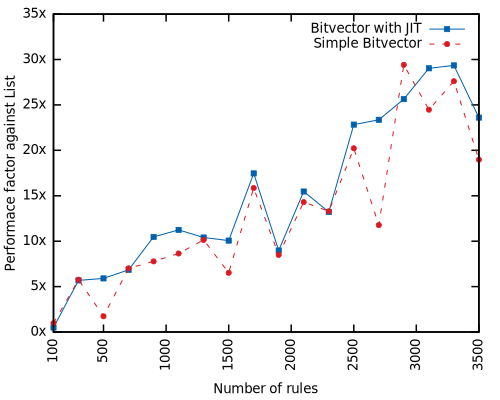
\includegraphics[width=\textwidth]{images/eval_w_relative}
        \caption{Relative matching performance (measured against the List algorithm).}
        \label{fig:eval_bad_case_relative}
    \end{subfigure}
    ~
    \begin{subfigure}{.32\linewidth}
        \centering
        \includegraphics[width=\textwidth]{images/eval_time}
        \caption{Time needed to insert rules into the switch.}
        \label{fig:eval-times}
    \end{subfigure}
    ~
    \begin{subfigure}{.32\linewidth}
        \centering
        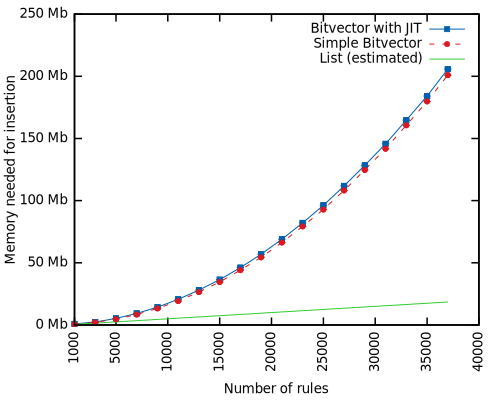
\includegraphics[width=\textwidth]{images/eval_mem}
        \caption{Memory needed to store rules in the switch. List memory is estimated.}
        \label{fig:eval-mem}
    \end{subfigure}
    \caption{An overview over the evaluation results.}
    \vspace{-0.5cm}
\end{figure*}

\subsubsection{Insertion Time}
\label{sec:eval-ins}
Figure~\ref{fig:eval-times} shows the significant loss in efficiency when inserting rules into the code generating algorithm.
The two graphs show the duration of an update with different sized rule sets in the 
JIT implementation and in the conventional bitvector approach.
Unfortunately, adding rules with the \textit{dpctl} tool is relatively slow itself, so that measurements using this tool
are too uncertain for measuring the algorithms' insertion performance.
Therefore, this test was executed on the two modules separately and in only one matching dimension.
In order to compensate for the decreased complexity of this approach compared to the full OpenFlow matching,
a greater number of rules was inserted into each matching engine.
Due to the requirement that the matching engine has to be operable 
immediately after every update operation, every insertion implies a complete regeneration of the JIT code.
That behaviour induces the massive additional update time seen in the measured data.
%A reduction might be possible by waiting if the next update is immediately following
%and, if true, waiting for the JIT regeneration until no more updates arrive for a certain time.
%The downside of this approach is the incorrect state of the JIT until it is rebuilt.
%Therefore, this approach only really works when inserting a big amout of rules while not classifying any packets.

\subsubsection{Memory Usage}
An increased memory consumption is the trade-off for using the bitvector implementation
instead of the list based lookup.
Figure~\ref{fig:eval-mem} shows a crude estimate of the difference.
The data for the two bitvector implementations was obtained by measuring memory consumption of the separate implementation
similar to Section~\ref{sec:eval-ins}.
The memory consumption of the list implementation is based on source code analysis.
Even though this method implies an uncertainty, it is sufficient to recognize the difference in magnitudes.
The small overhead of the JIT implementation in comparison with the simple bitvector approach
arises from the size of the actual JIT compiled function.

\section{Conclusion and Future Work}
The implementation of sophisticated algorithms in the OpenFlow reference switch indicates a gain in packet classification performance.
The bitvector algorithm itself achieves an impressive gain in classification 
performance in comparison to the previously used linear lookup.
Further optimization resulted in the development of a just-in-time compiler 
that generates a special function for looking up values in a given rule set.
Evaluation results show another increase of lookup performance for the JIT optimized algorithm.
However, the insertion time grows drastically for larger rule sets because 
of the time needed to regenerate the JIT compiled function for each new rule.

The evaluation also indicates that the prize to pay for faster classification 
is an increased usage of memory compared to the list implementation.
However, the JIT solution is in the same magnitude of memory consumption 
compared to the simple bitvector implementation. 
Another new benefit is the possibility to perform parallel lookups for each header dimension.
Only the bitvector aggregation step has to take place on one single node.

One of the main objectives for further optimization is the matching algorithm.
One possibility to speed this up is to reduce the JIT code update time.
Modifying the existing JIT function instead of deleting the old one and building 
a new one might be a worthwhile task.
Especially in environments with fast-changing rule sets that idea may offer 
a significant advantage over the current implementation.

Another idea that comes to mind is to implement a heuristic which detects 
the most popular flows of the last time span in an operating switch.
After gathering traffic data for a while, it might prove beneficial to tune 
the JIT function in such a way that the search for packet header data in a popular flow returns faster.

%eo text
\vspace{-0.3cm}
\balance

% trigger a \newpage just before the given reference
% number - used to balance the columns on the last page
% adjust value as needed - may need to be readjusted if
% the document is modified later
%\IEEEtriggeratref{8}
% The "triggered" command can be changed if desired:
%\IEEEtriggercmd{\enlargethispage{-5in}}

% references section

% can use a bibliography generated by BibTeX as a .bbl file
% BibTeX documentation can be easily obtained at:
% http://www.ctan.org/tex-archive/biblio/bibtex/contrib/doc/
% The IEEEtran BibTeX style support page is at:
% http://www.michaelshell.org/tex/ieeetran/bibtex/
\bibliographystyle{IEEEtranS}
% argument is your BibTeX string definitions and bibliography database(s)
%%%\bibliography{IEEEabrv,references,rfc}
\bibliography{IEEEabrv,references-short,rfc-short,paper-build/conferences-crossref-short}
%
% <OR> manually copy in the resultant .bbl file
% set second argument of \begin to the number of references
% (used to reserve space for the reference number labels box)
%\begin{thebibliography}{1}

%\bibitem{IEEEhowto:kopka}
%H.~Kopka and P.~W. Daly, \emph{A Guide to \LaTeX}, 3rd~ed.\hskip 1em plus
%  0.5em minus 0.4em\relax Harlow, England: Addison-Wesley, 1999.

%\end{thebibliography}




% that's all folks
\end{document}


